\chapter{Geometry is a positive semidefinite matrix that varies from point to point}\label{ch05}

% Standalone-build stubs for cross-chapter labels. Active only when this chapter is
% compiled alone through drivers/ch05.tex (jobname ch05), never in main.tex.
\makeatletter
\ifdefined\pdfstrcmp\ifnum\pdfstrcmp{\jobname}{ch05}=0
  \begingroup
  \def\omp@stub#1#2{\setcounter{chapter}{#2}\addtocounter{chapter}{-1}\refstepcounter{chapter}\label{#1}}
  \omp@stub{ch01}{1}\omp@stub{ch02}{2}\omp@stub{ch03}{3}\omp@stub{ch04}{4}
  \omp@stub{ch06}{6}\omp@stub{ch07}{7}\omp@stub{ch08}{8}\omp@stub{ch11}{11}
  \endgroup
  \setcounter{chapter}{5}
\fi\fi
\makeatother
\chaptermark{Geometry}

Every result in the Geometric series and in Observation Theory measures something. A cost, a distortion, a distance to an ideal, or the separation of two attention patterns. Each of those measurements that is smooth and smallest at zero error is, to second order, a quadratic form $\delta\T G\,\delta$ for some positive semidefinite matrix $G$. This chapter is about where that matrix comes from and what changes when it depends on where you stand.

The plan is short. A constant positive definite $G$ gives the Mahalanobis distance. A $G(x)$ that varies smoothly with position is a Riemannian metric, and distances become lengths of shortest curves. A map $C$ carries a metric on its output back to its input as $J\T G J$, and that pullback is the read operator of Observation Theory. Its kernel is the set of directions the map cannot see. Fisher information is the metric that KL divergence induces. Covariance matrices, hierarchies and graphs each come with a geometry of their own, and the last section explains why the angle of a spectral embedding carries graph distance while its radius carries density.

Everything is done in coordinates on $\R^n$ or on an open subset of it. The reader who wants the intrinsic theory of manifolds will find it in Lee~\cite{lee2018}. We use the facts, not the machinery.

%======================================================================
\section{A constant metric is a positive definite matrix, and the Mahalanobis distance is its distance}\label{sec:ch05:mahalanobis}

A \emph{metric} on a set is a rule $d(x,y)$ for the distance between two points. It must be nonnegative, zero only when $x=y$, symmetric, and it must obey the triangle inequality. A \emph{norm} on $\R^n$ is a length $\norm{v}$ that is positive for $v\ne 0$, scales as $\norm{cv}=\abs{c}\norm{v}$, and obeys $\norm{u+v}\le\norm{u}+\norm{v}$. Every norm gives a metric by $d(x,y)=\norm{x-y}$.

\begin{definition}[Metric and inner-product norm]\label{def:ch05:metric}
A function $d$ on pairs of points is a metric when, for all $x,y,z$,
\begin{equation}\label{eq:ch05:metric-axioms}
d(x,y)\ge 0,\qquad d(x,y)=0\iff x=y,\qquad d(x,y)=d(y,x),\qquad d(x,z)\le d(x,y)+d(y,z).
\end{equation}
For a symmetric positive definite matrix $G$, the inner product $\inner{u}{v}_G=u\T G v$ gives the norm and metric
\begin{equation}\label{eq:ch05:Gnorm}
\norm{v}_G=\sqrt{v\T G v},\qquad d_G(x,y)=\sqrt{(x-y)\T G\,(x-y)}.
\end{equation}
\end{definition}

Not every norm comes from an inner product. The $\ell_1$ norm $\sum_i\abs{v_i}$ and the $\ell_\infty$ norm $\max_i\abs{v_i}$ are norms whose unit balls are a diamond and a square. Their corners mean that the length of a small step depends on its direction in a way no matrix can express. The programme works almost entirely with norms of the form \eqref{eq:ch05:Gnorm}, for a reason that recurs in this chapter. A smooth cost that is zero at a point and has zero gradient there is, to second order, a quadratic form $\tfrac12\delta\T H\delta$, and $H$ is positive semidefinite at a minimum. So inner-product norms are what local analysis produces for any cost that is twice differentiable at its minimum, whatever the cost does far away. The smoothness is needed. The cost $\norm{\delta}_1$ is zero at the origin and has no quadratic expansion there. Where $H$ is singular the quadratic term is silent along $\ker H$, and higher-order terms decide.

Positive definiteness is what makes $d_G(x,y)=0$ force $x=y$. If $G$ is only positive semidefinite, two different points whose difference lies in $\ker G$ are at distance zero. Then $d_G$ is a \emph{pseudometric}, and we will see in \cref{sec:ch05:pullback} that this is not a defect. It is how a metric records what an observer ignores.

The most used choice is $G=\Sigma^{-1}$, the inverse of a covariance matrix. This is the Mahalanobis distance.
\begin{equation}\label{eq:ch05:mahalanobis}
d_M(x,y)=\sqrt{(x-y)\T\Sigma^{-1}(x-y)}=\norm{\Sigma^{-1/2}(x-y)}.
\end{equation}
The second form says that the Mahalanobis distance is the Euclidean distance after \emph{whitening}, that is, after the change of variables $z=\Sigma^{-1/2}x$ that turns the covariance into the identity. In the eigenbasis of $\Sigma=\sum_i\lambda_i e_ie_i\T$ it reads $d_M^2=\sum_i \big(e_i\T(x-y)\big)^2/\lambda_i$. A displacement along a direction of large variance is cheap and one along a direction of small variance is expensive. The unit ball $\{x:d_M(x,0)\le1\}$ is an ellipse with semi-axis $\sqrt{\lambda_i}$ along $e_i$.

\begin{example}[Two points at the same Euclidean distance]\label[example]{ex:ch05:mahal}
Let $\Sigma=\begin{pmatrix}2&1\\1&2\end{pmatrix}$. Its eigenvalues are $3$ along $(1,1)/\sqrt2$ and $1$ along $(1,-1)/\sqrt2$, and
\[
\Sigma^{-1}=\tfrac13\begin{pmatrix}2&-1\\-1&2\end{pmatrix}.
\]
Take $a=(1,1)$ and $b=(1,-1)$. Both have Euclidean length $\sqrt2$. In the Mahalanobis metric,
\[
d_M(a,0)^2=\tfrac13(2-2+2)=\tfrac23,\qquad d_M(b,0)^2=\tfrac13(2+2+2)=2,
\]
so $d_M(a,0)=0.816$ and $d_M(b,0)=1.414$. The point $a$ lies along the correlation, where the data spread is wide, and it is less surprising. The point $b$ goes against the correlation. \Cref{fig:ch05:ellipse} shows the unit Mahalanobis ellipse with both points.
\end{example}

\begin{figure}[t]
\centering
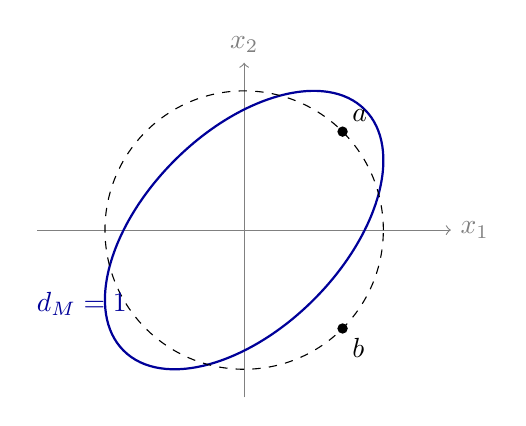
\begin{tikzpicture}[scale=1.25]
\draw[->,gray] (-2.1,0)--(2.1,0) node[right]{$x_1$};
\draw[->,gray] (0,-1.7)--(0,1.7) node[above]{$x_2$};
\draw[thick,blue!60!black,rotate=45] (0,0) ellipse ({sqrt(3)} and 1);
\draw[dashed] (0,0) circle ({sqrt(2)});
\fill (1,1) circle (1.5pt) node[above right]{$a$};
\fill (1,-1) circle (1.5pt) node[below right]{$b$};
\node[blue!60!black] at (-1.65,-0.75) {$d_M=1$};
\end{tikzpicture}
\caption{The unit ball of the Mahalanobis metric for $\Sigma$ of \cref{ex:ch05:mahal} (solid ellipse) and the Euclidean circle of radius $\sqrt2$ (dashed). Both points lie on the circle. Only $a$ lies inside the ellipse.}
\label{fig:ch05:ellipse}
\end{figure}

The Mahalanobis distance is the first instance of the chapter's theme. The data, through $\Sigma$, chose the metric. A consumer, an evaluator or a channel will choose it in later sections. \Cref{ch02} derives the same quadratic form as the exponent of a Gaussian density, and \cref{sec:ch05:fisher} shows that it is also the Fisher metric of a Gaussian location family.

\inproject{\path{geometric-methods/chapters/chapter-02-mahalanobis-distance.md}, section 2.1, uses $d_M$ with a hand-built $\Sigma$ on a nine-dimensional decision space. Chapter 7 of the same book builds path costs on a decision graph from Mahalanobis edge weights.}

\buildson{Primer L, section L.6 (quadratic forms and positive semidefinite matrices) and L.7 (eigenvectors) of \emph{Data Mining as Observation}.}
\usedin{\Cref{sec:ch05:fisher}, \cref{ch08} (evaluation as distance to an ideal), \cref{ch06}.}

%======================================================================
\section{A Riemannian metric is a positive definite matrix that varies smoothly, and distance is the length of the shortest curve}\label{sec:ch05:riemann}

On a curved surface no single matrix $G$ works everywhere. The fix is to let $G$ depend on the point. At each $x$ we have a positive definite matrix $G(x)$, and it prices small displacements $dx$ at that point as $dx\T G(x)\,dx$. The length of a curve is the sum of the prices of its small steps.

\begin{definition}[Riemannian metric, length, distance]\label{def:ch05:riemann}
A Riemannian metric on an open set $U\subseteq\R^n$ is a smooth map $x\mapsto G(x)$ into the symmetric positive definite matrices. A curve $\gamma:[0,1]\to U$ has length
\begin{equation}\label{eq:ch05:length}
L(\gamma)=\int_0^1\sqrt{\dot\gamma(t)\T\,G\big(\gamma(t)\big)\,\dot\gamma(t)}\;dt,
\end{equation}
and the distance between two points is the least length of a curve that joins them,
\begin{equation}\label{eq:ch05:geodist}
d_G(x,y)=\inf\{L(\gamma)\,:\,\gamma(0)=x,\ \gamma(1)=y\}.
\end{equation}
A curve that is locally length-minimizing, traced at constant speed, is a \emph{geodesic}.
\end{definition}

The length \eqref{eq:ch05:length} does not depend on how fast the curve is traced. Reparametrizing $t$ changes $\dot\gamma$ and $dt$ by reciprocal factors. When $G$ is constant and $U$ is convex, the shortest curve is the straight segment and $d_G$ is the distance \eqref{eq:ch05:Gnorm}. If $U$ is not convex the segment may leave it, and the shortest curve inside $U$ is longer. So the Mahalanobis distance is the flat case of \eqref{eq:ch05:geodist}. Geodesics in general solve a second-order ODE, the geodesic equation, which we will not need. Lee~\cite[ch.~4--6]{lee2018} derives it.

Where does a varying $G$ come from in practice? Usually from coordinates. Suppose a surface is described by a map $X(u)$ from parameters $u\in\R^k$ into $\R^n$, and lengths are measured in $\R^n$ in the ordinary way. A small step $du$ moves the point by $J\,du$ with $J=\partial X/\partial u$, and its squared length is $du\T J\T J\,du$. So the metric in the parameters is
\begin{equation}\label{eq:ch05:induced}
G(u)=J(u)\T J(u).
\end{equation}

\begin{example}[Polar coordinates and the sphere]\label[example]{ex:ch05:sphere}
For polar coordinates $X(r,\varphi)=(r\cos\varphi,r\sin\varphi)$ the Jacobian is $\begin{pmatrix}\cos\varphi&-r\sin\varphi\\ \sin\varphi&r\cos\varphi\end{pmatrix}$, and \eqref{eq:ch05:induced} gives $G=\diag(1,r^2)$. A radial step $dr$ costs $dr^2$. An angular step $d\varphi$ costs $r^2d\varphi^2$, so the same change of angle is a longer move far from the origin. Radius and angle are orthogonal coordinates, since $G$ has no off-diagonal term.

On the unit sphere with colatitude $\theta$ and longitude $\varphi$, $X=(\sin\theta\cos\varphi,\sin\theta\sin\varphi,\cos\theta)$ and \eqref{eq:ch05:induced} gives $G=\diag(1,\sin^2\theta)$. Take two points on the circle of colatitude $\theta=60^\circ$, a quarter turn apart in longitude. Walking along the circle of latitude, $\dot\theta=0$ and \eqref{eq:ch05:length} gives
\[
L_{\text{lat}}=\int_0^{\pi/2}\sin\theta\;d\varphi=\tfrac{\sqrt3}{2}\cdot\tfrac{\pi}{2}=1.360.
\]
The geodesics of the sphere are great circles, and the great-circle distance between unit vectors $p,q$ is the angle between them, $\arccos(p\T q)$. Here $p=(\tfrac{\sqrt3}2,0,\tfrac12)$ and $q=(0,\tfrac{\sqrt3}2,\tfrac12)$, so $p\T q=\tfrac14$ and
\[
d_{\text{sphere}}(p,q)=\arccos\tfrac14=1.318<1.360.
\]
The latitude circle is not a geodesic. The straight chord through the ball, $\norm{p-q}=\sqrt{3/2}=1.225$, is shorter still, but it leaves the sphere. That ordering, chord then great circle then latitude, holds for any two distinct points on a circle of latitude, with the last two equal only on the equator.
\end{example}

\begin{figure}[tbp]
\centering
%% SPHERE
%% SPHERE
\begin{tikzpicture}[scale=2.2]
\fill[plight] (0,0) circle (1);
\draw[thick,pgray] (0,0) circle (1);
\draw[guide] (-0.707,-0.664) -- (-0.643,-0.720) -- (-0.574,-0.770) -- (-0.500,-0.814) -- (-0.423,-0.852) -- (-0.342,-0.883) -- (-0.259,-0.908) -- (-0.174,-0.925) -- (-0.087,-0.936) -- (0.000,-0.940) -- (0.087,-0.936) -- (0.174,-0.925) -- (0.259,-0.908) -- (0.342,-0.883) -- (0.423,-0.852) -- (0.500,-0.814) -- (0.574,-0.770) -- (0.643,-0.720) -- (0.707,-0.664) -- (0.766,-0.604) -- (0.819,-0.539) -- (0.866,-0.470) -- (0.906,-0.397) -- (0.940,-0.321) -- (0.966,-0.243) -- (0.985,-0.163) -- (0.996,-0.082) -- (1.000,0.000) -- (0.996,0.082) -- (0.985,0.163) -- (0.966,0.243) -- (0.940,0.321) -- (0.906,0.397) -- (0.866,0.470) -- (0.819,0.539) -- (0.766,0.604) -- (0.707,0.664) -- (0.643,0.720) -- (0.574,0.770) -- (0.500,0.814) -- (0.423,0.852) -- (0.342,0.883) -- (0.259,0.908) -- (0.174,0.925) -- (0.087,0.936) -- (0.000,0.940) -- (-0.087,0.936) -- (-0.174,0.925) -- (-0.259,0.908) -- (-0.342,0.883) -- (-0.423,0.852) -- (-0.500,0.814) -- (-0.574,0.770) -- (-0.643,0.720) -- (-0.707,0.664) -- (-0.766,0.604) -- (-0.819,0.539) -- (-0.866,0.470) -- (-0.906,0.397) -- (-0.940,0.321) -- (-0.966,0.243) -- (-0.985,0.163) -- (-0.996,0.082) -- (-1.000,0.000) -- (-0.996,-0.082) -- (-0.985,-0.163) -- (-0.966,-0.243) -- (-0.940,-0.321) -- (-0.906,-0.397) -- (-0.866,-0.470) -- (-0.819,-0.539) -- (-0.766,-0.604) -- (-0.707,-0.664);
\draw[pgray,thin] (-0.612,-0.404) -- (-0.557,-0.452) -- (-0.497,-0.496) -- (-0.433,-0.534) -- (-0.366,-0.567) -- (-0.296,-0.594) -- (-0.224,-0.615) -- (-0.150,-0.630) -- (-0.075,-0.640) -- (0.000,-0.643) -- (0.075,-0.640) -- (0.150,-0.630) -- (0.224,-0.615) -- (0.296,-0.594) -- (0.366,-0.567) -- (0.433,-0.534) -- (0.497,-0.496) -- (0.557,-0.452) -- (0.612,-0.404) -- (0.663,-0.352) -- (0.709,-0.296) -- (0.750,-0.236) -- (0.785,-0.173) -- (0.814,-0.107) -- (0.837,-0.040) -- (0.853,0.030) -- (0.863,0.100) -- (0.866,0.171) -- (0.863,0.242) -- (0.853,0.312) -- (0.837,0.382) -- (0.814,0.449) -- (0.785,0.515) -- (0.750,0.578) -- (0.709,0.638) -- (0.663,0.694) -- (0.612,0.746) -- (0.557,0.794) -- (0.497,0.838) -- (0.433,0.876) -- (0.366,0.909) -- (0.296,0.936) -- (0.224,0.957) -- (0.150,0.972) -- (0.075,0.982) -- (0.000,0.985) -- (-0.075,0.982) -- (-0.150,0.972) -- (-0.224,0.957) -- (-0.296,0.936) -- (-0.366,0.909) -- (-0.433,0.876) -- (-0.497,0.838) -- (-0.557,0.794) -- (-0.612,0.746) -- (-0.663,0.694) -- (-0.709,0.638) -- (-0.750,0.578) -- (-0.785,0.515) -- (-0.814,0.449) -- (-0.837,0.382) -- (-0.853,0.312) -- (-0.863,0.242) -- (-0.866,0.171) -- (-0.863,0.100) -- (-0.853,0.030) -- (-0.837,-0.040) -- (-0.814,-0.107) -- (-0.785,-0.173) -- (-0.750,-0.236) -- (-0.709,-0.296) -- (-0.663,-0.352) -- (-0.612,-0.404);
\draw[very thick,porange] (-0.612,-0.404) -- (-0.579,-0.434) -- (-0.545,-0.461) -- (-0.509,-0.487) -- (-0.472,-0.511) -- (-0.433,-0.534) -- (-0.393,-0.554) -- (-0.352,-0.572) -- (-0.310,-0.589) -- (-0.268,-0.603) -- (-0.224,-0.615) -- (-0.180,-0.625) -- (-0.135,-0.633) -- (-0.091,-0.638) -- (-0.045,-0.642) -- (0.000,-0.643) -- (0.045,-0.642) -- (0.091,-0.638) -- (0.135,-0.633) -- (0.180,-0.625) -- (0.224,-0.615) -- (0.268,-0.603) -- (0.310,-0.589) -- (0.352,-0.572) -- (0.393,-0.554) -- (0.433,-0.534) -- (0.472,-0.511) -- (0.509,-0.487) -- (0.545,-0.461) -- (0.579,-0.434) -- (0.612,-0.404);
\draw[very thick,pgreen] (-0.612,-0.404) -- (-0.577,-0.418) -- (-0.541,-0.430) -- (-0.503,-0.442) -- (-0.465,-0.453) -- (-0.425,-0.463) -- (-0.385,-0.472) -- (-0.344,-0.480) -- (-0.303,-0.488) -- (-0.261,-0.494) -- (-0.218,-0.499) -- (-0.175,-0.504) -- (-0.131,-0.507) -- (-0.088,-0.510) -- (-0.044,-0.511) -- (0.000,-0.512) -- (0.044,-0.511) -- (0.088,-0.510) -- (0.131,-0.507) -- (0.175,-0.504) -- (0.218,-0.499) -- (0.261,-0.494) -- (0.303,-0.488) -- (0.344,-0.480) -- (0.385,-0.472) -- (0.425,-0.463) -- (0.465,-0.453) -- (0.503,-0.442) -- (0.541,-0.430) -- (0.577,-0.418) -- (0.612,-0.404);
\draw[thick,pred,dashed] (-0.612,-0.404) -- (0.612,-0.404);
\fill (-0.612,-0.404) circle (0.8pt) node[left,lbl] {$p$};
\fill (0.612,-0.404) circle (0.8pt) node[right,lbl] {$q$};
\fill (0.000,0.342) circle (0.6pt) node[above,lbl] {north pole};
\node[lbl,porange,right] at (1.15,0.25) {latitude path, $1.360$};
\node[lbl,pgreen,right] at (1.15,0.0) {great circle, $1.318$};
\node[lbl,pred,right] at (1.15,-0.25) {chord, $1.225$};
\end{tikzpicture}
\caption{Two points on the circle of colatitude $60^\circ$, a quarter turn apart, seen from above the northern hemisphere. The great circle (green) is shorter than the latitude path (orange), and the chord through the ball (red, dashed) is shorter still but leaves the sphere.}
\label{fig:ch05:sphere}
\end{figure}


A metric is attached to points, not to coordinates, so it must transform correctly when the coordinates change. Suppose new coordinates $z$ are related to old ones by $x=Az$ with $A$ invertible. A step $dz$ is the step $dx=A\,dz$, and its price must not change, so $dz\T G_z\,dz=dx\T G_x\,dx=dz\T A\T G_xA\,dz$ for every $dz$. Hence
\begin{equation}\label{eq:ch05:transform}
G_z=A\T G_x A .
\end{equation}
For a nonlinear change of coordinates the same rule holds pointwise with $A$ the Jacobian. Whitening is the case $G_x=\Sigma^{-1}$ and $A=\Sigma^{1/2}$, which gives $G_z=\Sigma^{1/2}\Sigma^{-1}\Sigma^{1/2}=I$. Equation \eqref{eq:ch05:induced} is the case $G_x=I$. The rule \eqref{eq:ch05:transform} also explains why eigenvalues of $G$ alone mean little. Rescaling a coordinate rescales them. Quantities that survive a change of coordinates, such as lengths, angles between curves, and the eigenvalues of $G_1^{-1}G_2$ for two metrics at the same point, are the ones with meaning.

The sphere example carries a lesson used throughout the programme. On $\R^n\setminus\{0\}$ write $x=r\,u$ with $r=\norm{x}$ and $u=x/\norm{x}$ on the unit sphere. The Euclidean metric splits as $dr^2+r^2\,du\T du$. Radius and direction are separate coordinates, and the distance between two directions is the angle $\arccos(u\T v)$. Cosine similarity is the cosine of that angle. Data Mining as Observation, section 0.6, introduces the sphere as the quotient that forgets length. Here it has acquired a metric.

\buildson{Multivariable calculus (arc length, Jacobians), \cref{sec:ch05:mahalanobis}.}
\usedin{\Cref{sec:ch05:pullback}, \cref{sec:ch05:laplacian}, \cref{ch07} (angle and norm in vector search).}

%======================================================================
\section{The read operator is a pullback metric, and its kernel defines the fibers of a quotient}\label{sec:ch05:pullback}

Equation \eqref{eq:ch05:induced} measured a parameter step by how far it moves a point in the output space. Nothing there required the output metric to be Euclidean or the map to be an embedding. That generality is the whole of the read operator.

\begin{definition}[Pullback metric]\label{def:ch05:pullback}
Let $C:U\subseteq\R^d\to\R^m$ be differentiable with Jacobian $J(x)=\partial C/\partial x$, and let $G(y)$ be a positive semidefinite metric on the output. The pullback of $G$ by $C$ is
\begin{equation}\label{eq:ch05:pullback}
P_C(x)=J(x)\T\,G\big(C(x)\big)\,J(x),\qquad \delta\T P_C(x)\,\delta=\norm{J(x)\,\delta}^2_{G(C(x))}.
\end{equation}
It is symmetric and positive semidefinite. Its kernel is $\ker P_C(x)=\ker\big(G^{1/2}J(x)\big)$, which equals $\ker J(x)$ when $G\pd0$.
\end{definition}

The second form in \eqref{eq:ch05:pullback} says what $P_C$ means. It prices an input displacement $\delta$ by how far it moves the output, measured in the output's own metric. This is exactly the read operator of Data Mining as Observation, equation 0.11, and of the shared notation of this book. Observation Theory states it as ``Observation Theory is pullback geometry''. The object is classical. Pullback metrics are standard Riemannian geometry~\cite{lee2018}, and with $G$ the Fisher metric the construction is Rao and Amari's information geometry~\cite{amari2016}. Averaged over a workload, $\bar P_{C,\mu}=\E_\mu[P_C(x)]$ is the active-subspace matrix of Constantine~\cite{constantine2015}. The programme's own assessment, \path{geometric-observation/articles/2026-10-01-ot-novelty-assessment.md}, credits these parents. What Observation Theory adds is the use of this one pullback across compression, retrieval and estimation, and \cref{ch06} sets out what is and is not new.

The metric $P_C$ is usually degenerate, and that is the point. A displacement $\delta$ in $\ker P_C(x)$ moves the output by zero to first order. The consumer cannot see it to first order. A finite step can still change the output. The consumer $C(x)=x_1^2$ has $J=0$ at the origin, so its kernel there is everything, yet the step $\delta=(0.1,0)$ changes the output by $0.01$.

\begin{definition}[Fibers and the observer's quotient]\label{def:ch05:quotient}
Two inputs are \emph{consumer-equivalent} when the consumer gives them the same output,
\begin{equation}\label{eq:ch05:quotient}
x\sim_C x'\iff C(x)=C(x').
\end{equation}
The equivalence classes are the \emph{fibers} $C^{-1}(y)$, and the set of classes is the quotient $U/\!\sim_C$. Near a point where $\rank J$ is constant and equal to $r$, the fiber through $x$ is a smooth surface of dimension $d-r$ whose tangent space is $\ker J(x)$.
\end{definition}

The last sentence is the constant-rank theorem. In the programme it is part (a) of the theorem ``Observer representation'' in \path{geometric-observation/paper/observer-representation.tex}. Pointwise, the kernel of the degenerate metric is the tangent to the fiber. Moving along a fiber costs nothing in the pullback metric because the consumer's output does not change. The quotient is the space the consumer actually lives on. Where $\rank J$ is constant and $G\pd0$, $P_C$ is a genuine, nondegenerate metric on it. Where the rank drops, as at the origin of the consumer $x_1^2$ above, the quotient need not be smooth there.

\begin{example}[A linear consumer]\label[example]{ex:ch05:linear}
Let $C(x)=x_1+2x_2$ with $G=1$. Then $J=(1\ \ 2)$ and
\[
P_C=J\T J=\begin{pmatrix}1&2\\2&4\end{pmatrix},
\]
with eigenvalues $5$ and $0$. The kernel is spanned by $(2,-1)$, and indeed $C(x+t(2,-1))=C(x)+t(2-2)=C(x)$. The fibers are the parallel lines $x_1+2x_2=c$, and the quotient is a single real line, parametrized by $c$. The displacement $\delta=(1,2)$ has $\delta\T P_C\delta=25=(J\delta)^2$.
\end{example}

\begin{example}[The angle reader is blind to radius]\label[example]{ex:ch05:normalize}
Let $C(x)=x/\norm{x}$, the map to the unit sphere, with the Euclidean metric on the output. Differentiating gives $J(x)=(I-uu\T)/r$ with $r=\norm{x}$ and $u=x/r$. At $x=(3,4)$, $r=5$ and $u=(0.6,0.8)$, so
\[
P_C=\frac{I-uu\T}{25}=\begin{pmatrix}0.0256&-0.0192\\-0.0192&0.0144\end{pmatrix}.
\]
Then $P_Cu=0$. The radial direction is the kernel, and the fibers are the open rays from the origin. The tangential unit vector $v=(-0.8,0.6)$ has $v\T P_Cv=1/25=0.04$, so a tangential step of length $\epsilon$ moves the direction by $\epsilon/5$. This is the polar metric of \cref{ex:ch05:sphere} with the radial term deleted and the angular term divided by $r^2$. The quotient by positive scaling is the sphere.
\end{example}

\begin{figure}[tbp]
\centering
\begin{tikzpicture}[scale=0.95]
\begin{scope}
\clip (-2,-2) rectangle (2,2);
\foreach \c in {-4,-3,-2,-1,0,1,2,3,4} {\draw[pgray,thin] ({\c-2*(-2)},-2) -- ({\c-2*2},2);}
\end{scope}
\draw[pgray] (-2,-2) rectangle (2,2);
\draw[vec,porange] (0,0) -- (0.447,0.894) node[above right,lbl] {$\nabla C$};
\draw[vec,pred] (0,0) -- (0.894,-0.447) node[below right,lbl,fill=white,inner sep=1pt] {$\ker P_C$};
\node[lbl,fill=white,inner sep=1pt] at (-0.9,-1.7) {fibers $x_1+2x_2=c$};
\node[lbl] at (0,-2.4) {(a) linear consumer};
\begin{scope}[xshift=5.2cm]
\foreach \a in {0,30,...,330} {\draw[pgray,thin] (0,0) -- (\a:2);}
\draw[pgray] (0,0) circle (2);
\fill (36.87:1.5) circle (1.6pt) node[left,lbl] {$x$};
\draw[vec,pred] (36.87:1.5) -- ++(36.87:0.7) node[right,lbl,fill=white,inner sep=1pt] {radial, unread};
\draw[vec,porange] (36.87:1.5) -- ++(126.87:0.7) node[above left,lbl,fill=white,inner sep=1pt] {tangential, read};
\node[lbl] at (0,-2.4) {(b) angle reader $x/\norm{x}$};
\end{scope}
\end{tikzpicture}
\caption{The kernel of the pullback metric is tangent to the fibers. For the linear consumer of \cref{ex:ch05:linear} the fibers are parallel lines along $(2,-1)$. For the angle reader of \cref{ex:ch05:normalize} they are rays, and the quotient is the circle of directions.}
\label{fig:ch05:pullback}
\end{figure}


\begin{example}[Softmax reads differences of logits]\label[example]{ex:ch05:softmax}
For the softmax output $p=\mathrm{softmax}(l)$ and KL divergence on the output, the metric on logits is $G=\diag(p)-pp\T$. With $p=(\tfrac12,\tfrac14,\tfrac14)$,
\[
G=\begin{pmatrix}\tfrac14&-\tfrac18&-\tfrac18\\[2pt]-\tfrac18&\tfrac3{16}&-\tfrac1{16}\\[2pt]-\tfrac18&-\tfrac1{16}&\tfrac3{16}\end{pmatrix},\qquad G\mathbf 1=0,\qquad \rank G=2.
\]
Adding the same constant to every logit leaves softmax unchanged, and $\mathbf 1$ is exactly the kernel. In \path{geometric-observation/paper/observation-theory.tex}, Proposition ``Softmax attention'', this kernel is why only the across-token demeaned key error reaches an attention head.
\end{example}

One caution belongs here, and Data Mining as Observation, section 0.6, gives its full form. The pointwise kernel $\ker P_C(x)$, the kernel of the workload average $\bar P_{C,\mu}$, and the global equivalence \eqref{eq:ch05:quotient} are three different objects. They agree for a linear consumer with a positive definite output metric. For the angle reader of \cref{ex:ch05:normalize} each $P_C(x)$ has a kernel, but the kernel turns with $x$, and the average over a spread of directions has no kernel at all. The consumer still identifies whole rays. A zero eigenvalue of the average is a statement about directions that are unread almost everywhere, not a description of the fibers.

\begin{example}[Averaging erases a turning kernel]\label[example]{ex:ch05:average}
Average the angle reader of \cref{ex:ch05:normalize} over a workload of two points, $x_1=(3,4)$ and $x_2=(4,-3)$, with equal weight. Both have radius $5$, and their directions $u_1=(0.6,0.8)$ and $u_2=(0.8,-0.6)$ are orthonormal. So $u_1u_1\T+u_2u_2\T=I$ and
\[
\bar P_{C,\mu}=\tfrac12\Big(\frac{I-u_1u_1\T}{25}+\frac{I-u_2u_2\T}{25}\Big)=\frac{I-\tfrac12I}{25}=\frac{I}{50}.
\]
Each pointwise operator has rank one with the radial direction as kernel. The average is a multiple of the identity and has no kernel. The averaged operator says the consumer reads every direction equally, which is true on average and false at every point.
\end{example}

\inproject{\path{geometric-observation/paper/observer-representation.tex}, Theorem ``Observer representation'' (a) and (b), states the fibers, the pullback $P_C=J\T GJ$, and $\ker P_C=\ker J$ for $G\pd0$. \path{geometric-observation/OBSERVATION.md} tabulates, consumer by consumer, what lies in $\ker P_C$ (``geodesic rank'' reads the angle and has the radius in its kernel).}

\buildson{\Cref{sec:ch05:riemann}, Data Mining as Observation sections 0.5 and 0.6, Primer L section L.4 (kernels).}
\usedin{\Cref{ch06} (the read operator and distortion $\tr(P_C\Sigma_\delta)$), \cref{ch07}, \cref{ch08} (the evaluator's pullback).}

%======================================================================
\section{Fisher information is the metric that KL divergence induces}\label{sec:ch05:fisher}

The KL divergence $\KL{p}{q}$ is not a metric. It is not symmetric and it fails the triangle inequality. But for two nearby members of a smooth family $p_\theta$ it is, to second order, a quadratic form in the parameter difference, and the matrix of that form is a Riemannian metric.

\begin{theorem}[KL is locally the Fisher metric]\label[theorem]{thm:ch05:fisher}
Let $p_\theta$ be a family of densities, twice differentiable in $\theta\in\R^k$, with Fisher information
\begin{equation}\label{eq:ch05:fisherinfo}
F(\theta)=\E_{p_\theta}\!\big[\nabla_\theta\log p_\theta(X)\,\nabla_\theta\log p_\theta(X)\T\big].
\end{equation}
Under the usual conditions for differentiating under the integral,
\begin{equation}\label{eq:ch05:klquad}
\KL{p_\theta}{p_{\theta+\delta}}=\tfrac12\,\delta\T F(\theta)\,\delta+o(\norm{\delta}^2).
\end{equation}
\end{theorem}

\begin{proof}
Write $\ell(\theta)=\log p_\theta(x)$ and expand $\ell(\theta+\delta)=\ell(\theta)+\delta\T\nabla\ell+\tfrac12\delta\T\nabla^2\ell\,\delta+o(\norm{\delta}^2)$. Then $\KL{p_\theta}{p_{\theta+\delta}}=-\E_\theta[\ell(\theta+\delta)-\ell(\theta)]$. The score has mean zero, $\E_\theta[\nabla\ell]=\int\nabla p_\theta=\nabla\!\int p_\theta=0$, so the linear term vanishes. The information identity $-\E_\theta[\nabla^2\ell]=F(\theta)$ turns the quadratic term into $\tfrac12\delta\T F\delta$.
\end{proof}

So $F(\theta)$ is a positive semidefinite matrix that varies with $\theta$, which is a Riemannian metric on the parameter space when it is positive definite. It is called the Fisher, or Fisher--Rao, metric~\cite{amari2016}. \Cref{ch02} develops $F$ as the curvature of the log-likelihood and the Cram\'er--Rao bound. Here the point is geometric. Locally, statistical distinguishability is a length. For distant parameters it is not, since the divergence is asymmetric and the Fisher distance is symmetric, so no function of the Fisher distance alone can equal both $\KL{p}{q}$ and $\KL{q}{p}$.

\begin{example}[Bernoulli family]\label[example]{ex:ch05:bernoulli}
For $p_\theta=\mathrm{Bernoulli}(\theta)$, $F(\theta)=1/\big(\theta(1-\theta)\big)$, which is $4$ at $\theta=0.5$. Move to $\theta=0.6$. The exact divergence is
\[
\KL{p_{0.5}}{p_{0.6}}=0.5\ln\tfrac{0.5}{0.6}+0.5\ln\tfrac{0.5}{0.4}=0.02041,
\]
and \eqref{eq:ch05:klquad} gives $\tfrac12\cdot4\cdot0.1^2=0.02$, about $2\%$ low. The reverse divergence is $\KL{p_{0.6}}{p_{0.5}}=0.6\ln1.2+0.4\ln0.8=0.02014$. The two directions agree to second order and differ at third order, which is why KL is not symmetric and still defines a symmetric metric locally. The metric blows up near $\theta=0$ and $\theta=1$, where a small change in a rare event's probability is easy to detect. The substitution $\theta=\sin^2\phi$ turns the metric into the constant $4\,d\phi^2$. So the Fisher distance between Bernoulli parameters is
\begin{equation}\label{eq:ch05:bernoulli-dist}
d_F(\theta_1,\theta_2)=2\,\big|\arcsin\sqrt{\theta_1}-\arcsin\sqrt{\theta_2}\big|,
\end{equation}
an angle. From $0.5$ to $0.9$ it is $2(1.2490-0.7854)=0.9273$.
\end{example}

\begin{example}[Gaussian location family]\label[example]{ex:ch05:gausslocation}
For $p_\mu=\Normal(\mu,\Sigma)$ with $\Sigma$ fixed, $F=\Sigma^{-1}$ for every $\mu$, and the expansion \eqref{eq:ch05:klquad} is exact, $\KL{p_\mu}{p_{\mu+\delta}}=\tfrac12\delta\T\Sigma^{-1}\delta$. The Fisher distance of the location family is the Mahalanobis distance \eqref{eq:ch05:mahalanobis}. With $\Sigma$ from \cref{ex:ch05:mahal} and $\delta=(0.3,-0.2)$, the divergence is $0.0633$.
\end{example}

\begin{figure}[tbp]
\centering
\begin{tikzpicture}
\begin{axis}[primer, xmin=-1.6, xmax=1.6, ymin=0.3, ymax=2.0, xlabel={mean $\mu$}, ylabel={standard deviation $\sigma$}, axis equal image]
\addplot[pblue, no marks] coordinates {(0.122,0.500) (0.124,0.516) (0.122,0.533) (0.115,0.548) (0.106,0.561) (0.094,0.572) (0.081,0.581) (0.067,0.588) (0.054,0.593) (0.040,0.596) (0.027,0.599) (0.013,0.600) (0.000,0.601) (-0.013,0.600) (-0.027,0.599) (-0.040,0.596) (-0.054,0.593) (-0.067,0.588) (-0.081,0.581) (-0.094,0.572) (-0.106,0.561) (-0.115,0.548) (-0.122,0.533) (-0.124,0.516) (-0.122,0.500) (-0.117,0.485) (-0.108,0.471) (-0.097,0.460) (-0.086,0.450) (-0.074,0.443) (-0.063,0.437) (-0.051,0.433) (-0.041,0.430) (-0.030,0.427) (-0.020,0.426) (-0.010,0.425) (-0.000,0.424) (0.010,0.425) (0.020,0.426) (0.030,0.427) (0.041,0.430) (0.051,0.433) (0.063,0.437) (0.074,0.443) (0.086,0.450) (0.097,0.460) (0.108,0.471) (0.117,0.485) (0.122,0.500)};
\addplot[pblue, no marks] coordinates {(0.245,1.000) (0.249,1.033) (0.244,1.065) (0.231,1.096) (0.211,1.122) (0.188,1.144) (0.161,1.161) (0.134,1.175) (0.107,1.185) (0.080,1.193) (0.053,1.198) (0.026,1.201) (0.000,1.202) (-0.026,1.201) (-0.053,1.198) (-0.080,1.193) (-0.107,1.185) (-0.134,1.175) (-0.161,1.161) (-0.188,1.144) (-0.211,1.122) (-0.231,1.096) (-0.244,1.065) (-0.249,1.033) (-0.245,1.000) (-0.233,0.969) (-0.216,0.942) (-0.195,0.919) (-0.172,0.901) (-0.149,0.886) (-0.125,0.875) (-0.103,0.866) (-0.081,0.859) (-0.060,0.855) (-0.040,0.851) (-0.020,0.850) (-0.000,0.849) (0.020,0.850) (0.040,0.851) (0.060,0.855) (0.081,0.859) (0.103,0.866) (0.125,0.875) (0.149,0.886) (0.172,0.901) (0.195,0.919) (0.216,0.942) (0.233,0.969) (0.245,1.000)};
\addplot[pblue, no marks] coordinates {(0.392,1.600) (0.398,1.652) (0.390,1.704) (0.369,1.753) (0.338,1.795) (0.300,1.830) (0.258,1.858) (0.215,1.880) (0.171,1.897) (0.128,1.909) (0.085,1.917) (0.042,1.921) (0.000,1.923) (-0.042,1.921) (-0.085,1.917) (-0.128,1.909) (-0.171,1.897) (-0.215,1.880) (-0.258,1.858) (-0.300,1.830) (-0.338,1.795) (-0.369,1.753) (-0.390,1.704) (-0.398,1.652) (-0.392,1.600) (-0.374,1.551) (-0.346,1.507) (-0.312,1.471) (-0.275,1.441) (-0.238,1.418) (-0.201,1.399) (-0.165,1.385) (-0.130,1.375) (-0.096,1.367) (-0.064,1.362) (-0.032,1.359) (-0.000,1.358) (0.032,1.359) (0.064,1.362) (0.096,1.367) (0.130,1.375) (0.165,1.385) (0.201,1.399) (0.238,1.418) (0.275,1.441) (0.312,1.471) (0.346,1.507) (0.374,1.551) (0.392,1.600)};
\addplot[pblue, no marks] coordinates {(1.122,0.500) (1.124,0.516) (1.122,0.533) (1.115,0.548) (1.106,0.561) (1.094,0.572) (1.081,0.581) (1.067,0.588) (1.054,0.593) (1.040,0.596) (1.027,0.599) (1.013,0.600) (1.000,0.601) (0.987,0.600) (0.973,0.599) (0.960,0.596) (0.946,0.593) (0.933,0.588) (0.919,0.581) (0.906,0.572) (0.894,0.561) (0.885,0.548) (0.878,0.533) (0.876,0.516) (0.878,0.500) (0.883,0.485) (0.892,0.471) (0.903,0.460) (0.914,0.450) (0.926,0.443) (0.937,0.437) (0.949,0.433) (0.959,0.430) (0.970,0.427) (0.980,0.426) (0.990,0.425) (1.000,0.424) (1.010,0.425) (1.020,0.426) (1.030,0.427) (1.041,0.430) (1.051,0.433) (1.063,0.437) (1.074,0.443) (1.086,0.450) (1.097,0.460) (1.108,0.471) (1.117,0.485) (1.122,0.500)};
\addplot[pblue, no marks] coordinates {(1.245,1.000) (1.249,1.033) (1.244,1.065) (1.231,1.096) (1.211,1.122) (1.188,1.144) (1.161,1.161) (1.134,1.175) (1.107,1.185) (1.080,1.193) (1.053,1.198) (1.026,1.201) (1.000,1.202) (0.974,1.201) (0.947,1.198) (0.920,1.193) (0.893,1.185) (0.866,1.175) (0.839,1.161) (0.812,1.144) (0.789,1.122) (0.769,1.096) (0.756,1.065) (0.751,1.033) (0.755,1.000) (0.767,0.969) (0.784,0.942) (0.805,0.919) (0.828,0.901) (0.851,0.886) (0.875,0.875) (0.897,0.866) (0.919,0.859) (0.940,0.855) (0.960,0.851) (0.980,0.850) (1.000,0.849) (1.020,0.850) (1.040,0.851) (1.060,0.855) (1.081,0.859) (1.103,0.866) (1.125,0.875) (1.149,0.886) (1.172,0.901) (1.195,0.919) (1.216,0.942) (1.233,0.969) (1.245,1.000)};
\addplot[pblue, no marks] coordinates {(1.392,1.600) (1.398,1.652) (1.390,1.704) (1.369,1.753) (1.338,1.795) (1.300,1.830) (1.258,1.858) (1.215,1.880) (1.171,1.897) (1.128,1.909) (1.085,1.917) (1.042,1.921) (1.000,1.923) (0.958,1.921) (0.915,1.917) (0.872,1.909) (0.829,1.897) (0.785,1.880) (0.742,1.858) (0.700,1.830) (0.662,1.795) (0.631,1.753) (0.610,1.704) (0.602,1.652) (0.608,1.600) (0.626,1.551) (0.654,1.507) (0.688,1.471) (0.725,1.441) (0.762,1.418) (0.799,1.399) (0.835,1.385) (0.870,1.375) (0.904,1.367) (0.936,1.362) (0.968,1.359) (1.000,1.358) (1.032,1.359) (1.064,1.362) (1.096,1.367) (1.130,1.375) (1.165,1.385) (1.201,1.399) (1.238,1.418) (1.275,1.441) (1.312,1.471) (1.346,1.507) (1.374,1.551) (1.392,1.600)};
\addplot[pblue, no marks] coordinates {(-0.878,0.500) (-0.876,0.516) (-0.878,0.533) (-0.885,0.548) (-0.894,0.561) (-0.906,0.572) (-0.919,0.581) (-0.933,0.588) (-0.946,0.593) (-0.960,0.596) (-0.973,0.599) (-0.987,0.600) (-1.000,0.601) (-1.013,0.600) (-1.027,0.599) (-1.040,0.596) (-1.054,0.593) (-1.067,0.588) (-1.081,0.581) (-1.094,0.572) (-1.106,0.561) (-1.115,0.548) (-1.122,0.533) (-1.124,0.516) (-1.122,0.500) (-1.117,0.485) (-1.108,0.471) (-1.097,0.460) (-1.086,0.450) (-1.074,0.443) (-1.063,0.437) (-1.051,0.433) (-1.041,0.430) (-1.030,0.427) (-1.020,0.426) (-1.010,0.425) (-1.000,0.424) (-0.990,0.425) (-0.980,0.426) (-0.970,0.427) (-0.959,0.430) (-0.949,0.433) (-0.937,0.437) (-0.926,0.443) (-0.914,0.450) (-0.903,0.460) (-0.892,0.471) (-0.883,0.485) (-0.878,0.500)};
\addplot[pblue, no marks] coordinates {(-0.755,1.000) (-0.751,1.033) (-0.756,1.065) (-0.769,1.096) (-0.789,1.122) (-0.812,1.144) (-0.839,1.161) (-0.866,1.175) (-0.893,1.185) (-0.920,1.193) (-0.947,1.198) (-0.974,1.201) (-1.000,1.202) (-1.026,1.201) (-1.053,1.198) (-1.080,1.193) (-1.107,1.185) (-1.134,1.175) (-1.161,1.161) (-1.188,1.144) (-1.211,1.122) (-1.231,1.096) (-1.244,1.065) (-1.249,1.033) (-1.245,1.000) (-1.233,0.969) (-1.216,0.942) (-1.195,0.919) (-1.172,0.901) (-1.149,0.886) (-1.125,0.875) (-1.103,0.866) (-1.081,0.859) (-1.060,0.855) (-1.040,0.851) (-1.020,0.850) (-1.000,0.849) (-0.980,0.850) (-0.960,0.851) (-0.940,0.855) (-0.919,0.859) (-0.897,0.866) (-0.875,0.875) (-0.851,0.886) (-0.828,0.901) (-0.805,0.919) (-0.784,0.942) (-0.767,0.969) (-0.755,1.000)};
\addplot[pblue, no marks] coordinates {(-0.608,1.600) (-0.602,1.652) (-0.610,1.704) (-0.631,1.753) (-0.662,1.795) (-0.700,1.830) (-0.742,1.858) (-0.785,1.880) (-0.829,1.897) (-0.872,1.909) (-0.915,1.917) (-0.958,1.921) (-1.000,1.923) (-1.042,1.921) (-1.085,1.917) (-1.128,1.909) (-1.171,1.897) (-1.215,1.880) (-1.258,1.858) (-1.300,1.830) (-1.338,1.795) (-1.369,1.753) (-1.390,1.704) (-1.398,1.652) (-1.392,1.600) (-1.374,1.551) (-1.346,1.507) (-1.312,1.471) (-1.275,1.441) (-1.238,1.418) (-1.201,1.399) (-1.165,1.385) (-1.130,1.375) (-1.096,1.367) (-1.064,1.362) (-1.032,1.359) (-1.000,1.358) (-0.968,1.359) (-0.936,1.362) (-0.904,1.367) (-0.870,1.375) (-0.835,1.385) (-0.799,1.399) (-0.762,1.418) (-0.725,1.441) (-0.688,1.471) (-0.654,1.507) (-0.626,1.551) (-0.608,1.600)};
\addplot[porange, dashed, domain=0:360, samples=60] ({0.2449*cos(x)},{1+0.1732*sin(x)});
\end{axis}
\end{tikzpicture}
\caption{Contours $\KL{\Normal(\mu_0,\sigma_0^2)}{\Normal(\mu,\sigma^2)}=0.03$ around nine base points. Each is nearly the ellipse of the Fisher metric $\diag(1/\sigma^2,2/\sigma^2)$, drawn dashed at $(0,1)$, and they grow in proportion to $\sigma$, so the same change of mean is easier to detect when the noise is small.}
\label{fig:ch05:fisher}
\end{figure}


The bridge to the read operator comes from composing \eqref{eq:ch05:klquad} with a map. Suppose an observation channel reads the input $x$ only through a consumer, so that the output law is $\kappa(\cdot\mid C(x))$ with Fisher metric $F(y)$ in $y$. Substituting $\delta_y=J\delta+o(\norm\delta)$ into \eqref{eq:ch05:klquad} gives
\begin{equation}\label{eq:ch05:bridge}
\KL{\kappa(\cdot\mid C(x+\delta))}{\kappa(\cdot\mid C(x))}=\tfrac12\,\delta\T J(x)\T F\big(C(x)\big)J(x)\,\delta+o(\norm{\delta}^2).
\end{equation}
The local divergence geometry of the channel, on the input space, is the read operator \eqref{eq:ch05:pullback} with the Fisher metric as $G$. For a Gaussian channel $\Normal(C(x),\sigma^2)$ with $C(x)=x_1+2x_2$ and $\sigma^2=0.25$, the expansion is exact. The step $\delta=(0.1,0.05)$ gives $J\delta=0.2$ and divergence $0.2^2/(2\cdot0.25)=0.08$.

\inproject{\path{geometric-observation/paper/observer-representation.tex}, Theorem ``Local Fisher bridge'', is \eqref{eq:ch05:bridge}. Its remark limits the claim. Global quantities such as $\MI{X}{W\mid S}$ are expectations of divergences, not averages of $P_C$, and the theorem says only that each local divergence is the read-operator quadratic form.}

\buildson{\Cref{sec:ch05:pullback}, \cref{ch02} (Fisher information), \cref{ch03} (KL divergence).}
\usedin{\Cref{ch06} (the local output metric $G$ of a KL consumer), \cref{ch08} (Dawid--Lauritzen decision geometry).}

%======================================================================
\section{Covariance matrices form a curved cone, and the affine-invariant distance measures ratios}\label{sec:ch05:spd}

A covariance matrix is a point in the set $\Sym^n_{++}$ of symmetric positive definite matrices. This set is an open cone inside the vector space $\Sym^n$ of symmetric matrices, of dimension $n(n+1)/2$. It is not a vector space. The difference of two covariances can be indefinite, and a straight line through two covariance matrices leaves the cone when extended. The Frobenius distance $\norm{S_1-S_2}_F$ is a valid metric but it measures differences, while for variances the natural scale is ratios. Doubling a variance from $1$ to $2$ and from $100$ to $200$ are the same change to the shape of a distribution.

\begin{definition}[Affine-invariant metric]\label{def:ch05:spd}
On $\Sym^n_{++}$ define the Riemannian metric on tangent directions $A,B\in\Sym^n$ at $S$ by
\begin{equation}\label{eq:ch05:aimetric}
\inner{A}{B}_S=\tr\big(S^{-1}A\,S^{-1}B\big).
\end{equation}
Its geodesic distance has the closed form
\begin{equation}\label{eq:ch05:aidist}
d_{AI}(S_1,S_2)=\big\|\log\big(S_1^{-1/2}S_2S_1^{-1/2}\big)\big\|_F=\Big(\sum_{i=1}^n\ln^2\lambda_i\Big)^{1/2},
\end{equation}
where $\lambda_i$ are the eigenvalues of $S_1^{-1}S_2$. It is invariant under every congruence by an invertible $A$,
\begin{equation}\label{eq:ch05:aiinv}
d_{AI}(AS_1A\T,AS_2A\T)=d_{AI}(S_1,S_2).
\end{equation}
\end{definition}

The closed form and the invariance are proved in Pennec, Fillard and Ayache~\cite{pennec2006}. The invariance is easy to see from \eqref{eq:ch05:aidist}, since $(AS_1A\T)^{-1}(AS_2A\T)=A^{-\mathsf T}S_1^{-1}S_2A\T$ is similar to $S_1^{-1}S_2$ and has the same eigenvalues. A change of units, a rotation or any invertible linear recoding of the variables leaves the distance between two covariances unchanged. In one dimension \eqref{eq:ch05:aidist} is $\abs{\ln(s_2/s_1)}$, the log-ratio.

\begin{example}[Ratios, not differences]\label[example]{ex:ch05:spd}
Take $S_1=I$, $S_2=\diag(4,\tfrac14)$ and $S_3=\diag(4,1)$. Then
\[
d_{AI}(I,S_2)=\sqrt{\ln^24+\ln^2\tfrac14}=\sqrt2\ln4=1.961,\qquad d_{AI}(I,S_3)=\ln4=1.386.
\]
The Frobenius distances are $\norm{I-S_2}_F=3.092$ and $\norm{I-S_3}_F=3$, almost equal. Frobenius sees the shrinking of the second variance from $1$ to $\tfrac14$ as a change of $0.75$. The affine-invariant metric sees it as a factor of four, as large as the growth of the first variance from $1$ to $4$.

For the invariance take $A=\begin{pmatrix}1&1\\0&1\end{pmatrix}$. Then $AA\T=\begin{pmatrix}2&1\\1&1\end{pmatrix}$ and $AS_2A\T=\begin{pmatrix}4.25&0.25\\0.25&0.25\end{pmatrix}$, and $d_{AI}$ between these two is again $1.961$. The Frobenius distance changes under the same map.

The geodesic midpoint of $S_1$ and $S_2$ is $S_1^{1/2}\big(S_1^{-1/2}S_2S_1^{-1/2}\big)^{1/2}S_1^{1/2}$, which for $I$ and $S_2$ is $\diag(2,\tfrac12)$, at distance $0.980$ from each end. Its determinant is $1$, the geometric mean of the two determinants. The arithmetic mean $\diag(2.125,0.625)$ is not the midpoint.
\end{example}

\begin{figure}[tbp]
\centering
\begin{tikzpicture}[scale=0.9]
\foreach \x/\a/\b [count=\i] in {0/1.000/1.000, 2.6/1.189/0.841, 5.2/1.414/0.707, 7.8/1.682/0.595, 10.4/2.000/0.500}
  {\draw[thick,pgreen,fill=pgreen!10] (\x,0) ellipse ({0.5*\a} and {0.5*\b});}
\foreach \x/\a/\b in {0/1.000/1.000, 2.6/1.323/0.901, 5.2/1.581/0.791, 7.8/1.803/0.661, 10.4/2.000/0.500}
  {\draw[thick,pblue,fill=pblue!10] (\x,-1.6) ellipse ({0.5*\a} and {0.5*\b});}
\foreach \x/\t in {0/0, 2.6/0.25, 5.2/0.5, 7.8/0.75, 10.4/1} {\node[lbl] at (\x,-2.5) {$t=\t$};}
\node[lbl,pgreen,align=right,left] at (-0.9,0) {affine-invariant\\$\det=1$ throughout};
\node[lbl,pblue,align=right,left] at (-0.9,-1.6) {Euclidean\\$\det$ up to $1.56$};
\end{tikzpicture}
\caption{Two paths from $I$ to $\diag(4,\tfrac14)$, drawn as covariance ellipses with semi-axes $\sqrt{\lambda_i}$. The affine-invariant geodesic keeps the determinant at one. The straight Euclidean path swells in the middle, where the determinant reaches $1.56$.}
\label{fig:ch05:spd}
\end{figure}


Two relatives are worth knowing. The \emph{log-Euclidean} distance $\norm{\log S_1-\log S_2}_F$ of Arsigny, Fillard, Pennec and Ayache~\cite{arsigny2007} maps the cone flat with the matrix logarithm. It equals $d_{AI}$ when $S_1$ and $S_2$ commute and in general differs otherwise, and it is cheaper because means have a closed form. The Fisher metric of the zero-mean Gaussian family $\Normal(0,S)$ is half of \eqref{eq:ch05:aimetric}, so that
\begin{equation}\label{eq:ch05:gausscov}
\KL{\Normal(0,S)}{\Normal(0,S+\epsilon A)}=\tfrac14\,\epsilon^2\tr\big((S^{-1}A)^2\big)+o(\epsilon^2).
\end{equation}
The affine-invariant geometry is therefore the information geometry of covariance, up to a constant factor~\cite{amari2016}. In one dimension, with $S=s$ and $A=s$, \eqref{eq:ch05:gausscov} reads $\KL{\Normal(0,s)}{\Normal(0,s(1+\epsilon))}\approx\epsilon^2/4$. A $10\%$ increase of variance costs exactly $\tfrac12(1/1.1-1+\ln1.1)=0.0022$ nats whether the variance is $1$ or $100$ (the quadratic approximation gives $0.0025$). This is the ratio property again, in information units.

\inproject{\path{geometric-methods/chapters/chapter-04-spd-manifolds.md} works with the log-Euclidean distance for frequency-band covariance trajectories of acoustic signals, and section 4.7 lists the affine-invariant metric as the congruence-invariant alternative.}

\buildson{\Cref{sec:ch05:riemann}, \cref{sec:ch05:fisher}, \cref{ch01} (matrix square roots and functions of symmetric matrices).}
\usedin{\Cref{ch06} (covariance of the source $\Sigma_x$ and of the error $\Sigma_\delta$), \cref{ch08} (the second moment that selects a budgeted read subspace).}

%======================================================================
\section{Hyperbolic space has room for trees}\label{sec:ch05:hyperbolic}

In the plane a circle of radius $\rho$ has circumference $2\pi\rho$. A balanced tree with branching factor $k$ has $k^\rho$ nodes at depth $\rho$. In a fixed dimension that room grows only polynomially, and polynomial room cannot hold exponentially many well-separated nodes, so a Euclidean embedding of a deep tree must crowd leaves together or stretch the tree. Hyperbolic space has exponential room. A circle of radius $\rho$ has circumference $2\pi\sinh\rho$, which for $\rho=3$ is $62.9$ against the Euclidean $18.8$.

\begin{definition}[Poincar\'e disk]\label{def:ch05:poincare}
The Poincar\'e disk is the open unit disk $\{x\in\R^2:\norm{x}<1\}$ with the metric
\begin{equation}\label{eq:ch05:poincare-metric}
G(x)=\Big(\frac{2}{1-\norm{x}^2}\Big)^{2}I.
\end{equation}
Its geodesic distance is
\begin{equation}\label{eq:ch05:poincare-dist}
d_{\mathbb H}(x,y)=\operatorname{arccosh}\!\Big(1+\frac{2\norm{x-y}^2}{(1-\norm{x}^2)(1-\norm{y}^2)}\Big),
\end{equation}
and from the origin $d_{\mathbb H}(0,x)=2\operatorname{artanh}\norm{x}=\ln\frac{1+\norm{x}}{1-\norm{x}}$. The same formulas define the Poincar\'e ball in $\R^n$.
\end{definition}

The metric \eqref{eq:ch05:poincare-metric} is the Euclidean one times a factor that depends only on the radius. Such a metric is called \emph{conformal}. It measures angles as Euclidean geometry does but stretches lengths, and the stretch grows without bound toward the rim. Geodesics are diameters and arcs of circles that meet the rim at right angles.

\begin{example}[Distances in the disk]\label[example]{ex:ch05:poincare}
From the origin, $d_{\mathbb H}(0,(0.5,0))=\ln3=1.099$ and $d_{\mathbb H}(0,(0.9,0))=\ln19=2.944$. Near the rim the conformal factor is $2/(1-0.81)=10.5$, so a Euclidean step of $0.01$ at radius $0.9$ has hyperbolic length about $0.105$.

Now take two points near the rim, $x=(0.9,0)$ and $y=(0,0.9)$, a quarter turn apart. Then $\norm{x-y}^2=1.62$ and
\[
d_{\mathbb H}(x,y)=\operatorname{arccosh}\!\Big(1+\frac{3.24}{0.0361}\Big)=\operatorname{arccosh}(90.75)=5.201.
\]
The path through the origin has length $2\ln19=5.889$, so the direct geodesic saves only $12\%$. In Euclidean terms the chord $1.273$ saves $29\%$ over the path through the origin of length $1.8$. In hyperbolic space the shortest route between two points near the rim bends toward the centre, as the path between two leaves of a tree passes through their common ancestor. \Cref{fig:ch05:poincare} draws the geodesic.
\end{example}

\begin{figure}[t]
\centering
\begin{tikzpicture}[scale=2.4]
\draw[thick] (0,0) circle (1);
\draw[very thick,pblue] (0.900,0.000) -- (0.895,0.001) -- (0.890,0.001) -- (0.885,0.002) -- (0.879,0.002) -- (0.873,0.003) -- (0.867,0.004) -- (0.860,0.005) -- (0.853,0.006) -- (0.846,0.007) -- (0.838,0.008) -- (0.830,0.010) -- (0.821,0.011) -- (0.812,0.013) -- (0.802,0.015) -- (0.792,0.017) -- (0.781,0.020) -- (0.769,0.023) -- (0.756,0.026) -- (0.742,0.029) -- (0.727,0.033) -- (0.711,0.038) -- (0.694,0.044) -- (0.675,0.050) -- (0.655,0.057) -- (0.632,0.066) -- (0.607,0.076) -- (0.580,0.088) -- (0.551,0.103) -- (0.518,0.120) -- (0.481,0.141) -- (0.440,0.167) -- (0.395,0.200) -- (0.345,0.240) -- (0.290,0.292) -- (0.229,0.358) -- (0.165,0.444) -- (0.099,0.557) -- (0.040,0.706) -- (0.000,0.900);
\draw[very thick,pblue] (-0.600,0.600) -- (-0.596,0.594) -- (-0.592,0.588) -- (-0.588,0.581) -- (-0.583,0.575) -- (-0.579,0.567) -- (-0.574,0.560) -- (-0.570,0.552) -- (-0.565,0.543) -- (-0.560,0.534) -- (-0.554,0.525) -- (-0.549,0.515) -- (-0.544,0.504) -- (-0.538,0.493) -- (-0.532,0.481) -- (-0.526,0.468) -- (-0.520,0.454) -- (-0.514,0.439) -- (-0.508,0.423) -- (-0.502,0.406) -- (-0.495,0.388) -- (-0.489,0.368) -- (-0.483,0.347) -- (-0.476,0.324) -- (-0.471,0.299) -- (-0.465,0.272) -- (-0.460,0.242) -- (-0.456,0.210) -- (-0.452,0.174) -- (-0.450,0.136) -- (-0.450,0.093) -- (-0.452,0.047) -- (-0.458,-0.004) -- (-0.467,-0.060) -- (-0.482,-0.122) -- (-0.503,-0.188) -- (-0.533,-0.260) -- (-0.574,-0.337) -- (-0.629,-0.418) -- (-0.700,-0.500);
\draw[very thick,pblue] (0.200,-0.850) -- (0.200,-0.844) -- (0.201,-0.838) -- (0.201,-0.831) -- (0.202,-0.825) -- (0.203,-0.818) -- (0.204,-0.810) -- (0.205,-0.802) -- (0.206,-0.794) -- (0.208,-0.786) -- (0.209,-0.777) -- (0.211,-0.768) -- (0.214,-0.758) -- (0.216,-0.748) -- (0.219,-0.737) -- (0.223,-0.726) -- (0.227,-0.714) -- (0.231,-0.702) -- (0.236,-0.689) -- (0.242,-0.675) -- (0.249,-0.661) -- (0.256,-0.646) -- (0.265,-0.630) -- (0.275,-0.614) -- (0.286,-0.597) -- (0.299,-0.579) -- (0.314,-0.561) -- (0.331,-0.542) -- (0.350,-0.522) -- (0.372,-0.502) -- (0.397,-0.483) -- (0.425,-0.463) -- (0.457,-0.445) -- (0.493,-0.427) -- (0.534,-0.412) -- (0.579,-0.399) -- (0.628,-0.390) -- (0.682,-0.387) -- (0.740,-0.390) -- (0.800,-0.400);
\draw[very thick,pblue] (-0.900,0.000) -- (-0.895,0.000) -- (-0.890,0.000) -- (-0.884,0.000) -- (-0.879,0.000) -- (-0.873,0.000) -- (-0.866,0.000) -- (-0.860,0.000) -- (-0.853,0.000) -- (-0.845,0.000) -- (-0.837,0.000) -- (-0.829,0.000) -- (-0.820,0.000) -- (-0.810,0.000) -- (-0.800,0.000) -- (-0.789,0.000) -- (-0.778,0.000) -- (-0.765,0.000) -- (-0.751,0.000) -- (-0.737,0.000) -- (-0.721,0.000) -- (-0.704,0.000) -- (-0.685,0.000) -- (-0.664,0.000) -- (-0.641,0.000) -- (-0.616,0.000) -- (-0.588,0.000) -- (-0.556,0.000) -- (-0.520,0.000) -- (-0.480,0.000) -- (-0.433,0.000) -- (-0.380,0.000) -- (-0.316,0.000) -- (-0.241,0.000) -- (-0.150,0.000) -- (-0.038,0.000) -- (0.103,0.000) -- (0.288,0.000) -- (0.539,0.000) -- (0.900,0.000);
\draw[porange,thick] (0.000,0.000) circle (0.0700);
\draw[porange,thick] (0.350,0.000) circle (0.0614);
\draw[porange,thick] (0.175,0.303) circle (0.0614);
\draw[porange,thick] (-0.175,0.303) circle (0.0614);
\draw[porange,thick] (-0.350,0.000) circle (0.0614);
\draw[porange,thick] (-0.175,-0.303) circle (0.0614);
\draw[porange,thick] (0.175,-0.303) circle (0.0614);
\draw[porange,thick] (0.600,0.000) circle (0.0448);
\draw[porange,thick] (0.520,0.300) circle (0.0448);
\draw[porange,thick] (0.300,0.520) circle (0.0448);
\draw[porange,thick] (0.000,0.600) circle (0.0448);
\draw[porange,thick] (-0.300,0.520) circle (0.0448);
\draw[porange,thick] (-0.520,0.300) circle (0.0448);
\draw[porange,thick] (-0.600,0.000) circle (0.0448);
\draw[porange,thick] (-0.520,-0.300) circle (0.0448);
\draw[porange,thick] (-0.300,-0.520) circle (0.0448);
\draw[porange,thick] (-0.000,-0.600) circle (0.0448);
\draw[porange,thick] (0.300,-0.520) circle (0.0448);
\draw[porange,thick] (0.520,-0.300) circle (0.0448);
\draw[porange,thick] (0.764,0.236) circle (0.0252);
\draw[porange,thick] (0.544,0.587) circle (0.0252);
\draw[porange,thick] (0.177,0.780) circle (0.0252);
\draw[porange,thick] (-0.236,0.764) circle (0.0252);
\draw[porange,thick] (-0.587,0.544) circle (0.0252);
\draw[porange,thick] (-0.780,0.177) circle (0.0252);
\draw[porange,thick] (-0.764,-0.236) circle (0.0252);
\draw[porange,thick] (-0.544,-0.587) circle (0.0252);
\draw[porange,thick] (-0.177,-0.780) circle (0.0252);
\draw[porange,thick] (0.236,-0.764) circle (0.0252);
\draw[porange,thick] (0.587,-0.544) circle (0.0252);
\draw[porange,thick] (0.780,-0.177) circle (0.0252);
\draw[porange,thick] (0.879,0.272) circle (0.0108);
\draw[porange,thick] (0.625,0.675) circle (0.0108);
\draw[porange,thick] (0.204,0.897) circle (0.0108);
\draw[porange,thick] (-0.272,0.879) circle (0.0108);
\draw[porange,thick] (-0.675,0.625) circle (0.0108);
\draw[porange,thick] (-0.897,0.204) circle (0.0108);
\draw[porange,thick] (-0.879,-0.272) circle (0.0108);
\draw[porange,thick] (-0.625,-0.675) circle (0.0108);
\draw[porange,thick] (-0.204,-0.897) circle (0.0108);
\draw[porange,thick] (0.272,-0.879) circle (0.0108);
\draw[porange,thick] (0.675,-0.625) circle (0.0108);
\draw[porange,thick] (0.897,-0.204) circle (0.0108);
\foreach \q in {(-0.6,0.6),(-0.7,-0.5),(0.2,-0.85),(0.8,-0.4),(-0.9,0)} {\fill[pblue] \q circle (0.5pt);}
\fill (0.9,0) circle (0.7pt) node[right,lbl]{$x$};
\fill (0,0.9) circle (0.7pt) node[above,lbl]{$y$};
\end{tikzpicture}
\caption{Hyperbolic geodesics in the Poincar\'e disk are diameters and arcs that meet the rim at right angles (blue). The arc from $x=(0.9,0)$ to $y=(0,0.9)$ lies on the circle with centre $(1.006,1.006)$ and radius $1.011$, and it bends toward the centre. The small orange circles all have the same size in the metric \eqref{eq:ch05:poincare-metric}, so their Euclidean radius shrinks like $1-\norm{x}^2$ toward the rim.}
\label{fig:ch05:poincare}
\end{figure}

Nickel and Kiela~\cite{nickel2017} train Poincar\'e-ball embeddings of hierarchies, such as the WordNet noun taxonomy, by gradient descent on \eqref{eq:ch05:poincare-dist}. In their experiments general nodes settle near the centre and specific ones near the rim.

The hyperbolic picture is a tool with a scope. The Keep-the-Angle project tested whether its emergent geometries are better described as hyperbolic, with controls, and rejected that hypothesis. The rejection is recorded in \path{the-angular-observer/README.md} (``the hyperbolic-reframe hypothesis was tested with controls and rejected'', script \path{hyperbolic.py}). A hierarchy suggests hyperbolic space. A manifold-like graph does not.

\inproject{\path{geometric-methods/chapters/chapter-03-hyperbolic-geometry.md}, section 3.2.2, implements \eqref{eq:ch05:poincare-dist} in its M\"obius-addition form with curvature parameter $c$, and section 3.3 embeds a taxonomy.}

\buildson{\Cref{sec:ch05:riemann}.}
\usedin{\Cref{ch07} (embeddings and their geometry).}

%======================================================================
\section{The graph Laplacian is a metric on functions, and its low eigenvectors embed the graph}\label{sec:ch05:laplacian}

A graph has no coordinates, so it has no metric in the sense of \cref{sec:ch05:riemann}. It has something close. For a function $f$ on the nodes, the sum of squared differences across edges measures how much $f$ varies. That quadratic form plays the role $\delta\T G\delta$ played above, with the graph supplying $G$.

\begin{definition}[Laplacian and its quadratic form]\label{def:ch05:laplacian}
For a graph with symmetric nonnegative weights $w_{ij}$, degrees $d_i=\sum_jw_{ij}$, $D=\diag(d)$ and adjacency $W$, the Laplacian is $L=D-W$, and
\begin{equation}\label{eq:ch05:laplacian}
f\T Lf=\tfrac12\sum_{i,j}w_{ij}(f_i-f_j)^2\ \ge\ 0.
\end{equation}
The normalized Laplacian is $\mathcal L=I-D^{-1/2}WD^{-1/2}$, and Data Mining as Observation, equation 0.19, introduces it.
\end{definition}

For the path $1-2-3$ and $f=(0,1,3)$, \eqref{eq:ch05:laplacian} is $(0-1)^2+(1-3)^2=5$. The Laplacian there is $\begin{pmatrix}1&-1&0\\-1&2&-1\\0&-1&1\end{pmatrix}$, with eigenvalues $0,1,3$. The constant vector has eigenvalue $0$. A smooth function has a small quadratic form and a rough one a large form.

Laplacian eigenmaps, due to Belkin and Niyogi~\cite{belkin2003}, turn this into coordinates. Seek points $y_i\in\R^m$, one per node, that keep joined nodes close, so that $\sum_{ij}w_{ij}\norm{y_i-y_j}^2$ is small. To rule out the trivial answer of all points equal, fix the scale with $Y\T DY=I$ and drop the constant solution. For a connected graph with every degree positive, the minimizers are the next eigenvectors of the generalized problem
\begin{equation}\label{eq:ch05:eigenmap}
L\,y=\lambda\,D\,y,\qquad 0=\lambda_1\le\lambda_2\le\cdots,
\end{equation}
and node $i$ gets coordinates $(y_2(i),\ldots,y_{m+1}(i))$. The eigenvalues of \eqref{eq:ch05:eigenmap} are those of the normalized Laplacian.

The derivation is a Lagrange-multiplier argument of the kind \cref{ch04} develops. With $Y$ the $n\times m$ matrix of coordinates, the objective is $\tfrac12\sum_{ij}w_{ij}\norm{y_i-y_j}^2=\tr(Y\T LY)$ by \eqref{eq:ch05:laplacian} applied to each column. Minimizing it subject to $Y\T DY=I$ with a symmetric multiplier matrix $\Lambda$ gives the stationarity condition
\begin{equation}\label{eq:ch05:eigenmap-kkt}
LY=DY\Lambda .
\end{equation}
Choosing a basis in which $\Lambda$ is diagonal turns \eqref{eq:ch05:eigenmap-kkt} into $m$ copies of \eqref{eq:ch05:eigenmap}, and the objective equals $\tr\Lambda$, the sum of the chosen eigenvalues. The smallest sum, with the constant solution excluded, takes the eigenvectors of the $m$ smallest nonzero eigenvalues. With $D$ replaced by $I$ the argument is the Rayleigh-quotient characterization of eigenvectors, and the pair $(L,D)$ is a matrix pencil in the sense of \cref{ch01}. Belkin and Niyogi motivate the construction by the Laplace--Beltrami operator of the manifold the data are sampled from, which the Laplacian of a neighbourhood graph approximates, so that the embedding is a picture of the manifold. Data Mining as Observation, section 0.10, covers the vocabulary, the commute-time scaling, and the path-graph example.

\begin{example}[The six-cycle embeds as a hexagon]\label[example]{ex:ch05:cycle}
The cycle $C_6$ has every degree $2$, so $\mathcal L=I-W/2$. Its eigenvalues are $1-\cos(2\pi k/6)$, namely $0,\ 0.5,\ 0.5,\ 1.5,\ 1.5,\ 2$. The eigenvalue $0.5$ has the eigenvectors $\cos(2\pi i/6)$ and $\sin(2\pi i/6)$. Using those as coordinates puts node $i$ at angle $60^\circ\cdot i$ on a circle. The angle between the embedded nodes $i$ and $j$ is $60^\circ$ times the hop distance $\min(\abs{i-j},6-\abs{i-j})$, exactly. Every node has the same radius. Any other orthonormal basis of the same eigenspace rotates or reflects the hexagon and leaves the angles unchanged.
\end{example}

\begin{figure}[tbp]
\centering
\begin{tikzpicture}[scale=1.25]
\coordinate (s0) at (0.250,0.794);
\coordinate (s1) at (0.551,-0.550);
\coordinate (s2) at (-0.400,0.747);
\coordinate (s3) at (-0.989,0.642);
\coordinate (s4) at (0.594,-0.064);
\coordinate (s5) at (-0.394,-0.443);
\coordinate (s6) at (-0.490,-0.110);
\coordinate (s7) at (0.009,0.107);
\coordinate (s8) at (0.991,0.585);
\coordinate (s9) at (0.244,0.978);
\coordinate (s10) at (-0.569,-0.680);
\coordinate (s11) at (0.225,-0.912);
\coordinate (e0) at (4.700,0.000);
\coordinate (e1) at (4.566,0.500);
\coordinate (e2) at (4.200,0.866);
\coordinate (e3) at (3.700,1.000);
\coordinate (e4) at (3.200,0.866);
\coordinate (e5) at (2.834,0.500);
\coordinate (e6) at (2.700,0.000);
\coordinate (e7) at (2.834,-0.500);
\coordinate (e8) at (3.200,-0.866);
\coordinate (e9) at (3.700,-1.000);
\coordinate (e10) at (4.200,-0.866);
\coordinate (e11) at (4.566,-0.500);
\foreach \i [evaluate=\i as \j using {int(mod(\i+1,12))}] in {0,...,11} {\draw[pgray] (s\i) -- (s\j); \draw[pblue,thick] (e\i) -- (e\j);}
\foreach \i in {0,...,11} {\fill[pblue] (s\i) circle (1.3pt); \fill[pblue] (e\i) circle (1.3pt);}
\draw[flow,porange] (1.3,0) -- (2.4,0) node[midway,above,lbl] {eigenmap};
\node[lbl] at (0,-1.35) {scrambled drawing};
\node[lbl] at (3.7,-1.35) {eigenmap embedding};
\end{tikzpicture}
\caption{The twelve-node ring drawn at random positions (left) and embedded by the two eigenvectors of its smallest nonzero Laplacian eigenvalue (right). The embedding recovers the circle, and the angle between neighbours is $30^\circ$.}
\label{fig:ch05:ring}
\end{figure}


In the cycle the angle is the geodesic and the radius says nothing, because every node has the same degree. On large, irregular graphs the same split happens for a reason that \cref{sec:ch05:angle} explains. We end this section with the effective resistance, which that argument needs. Treat each edge as a unit resistor. The effective resistance between nodes $i$ and $j$ is
\begin{equation}\label{eq:ch05:resistance}
R(i,j)=(e_i-e_j)\T L^{+}(e_i-e_j),
\end{equation}
with $L^+$ the pseudoinverse. On $C_6$ two nodes $k$ hops apart are joined by parallel paths of lengths $k$ and $6-k$, so $R=k(6-k)/6$, which is $5/6$, $4/3$ and $3/2$ for $k=1,2,3$. The commute-time embedding of Data Mining as Observation, equation 0.20, is the one whose squared Euclidean distances are exactly these resistances.

\inproject{\path{the-angular-observer/theorem.md}, section 1, defines the normalized Laplacian, the commute embedding $\Psi_i=\big(u_k(i)/\sqrt{\lambda_kd_i}\big)_{k\ge2}$ with $\norm{\Psi_i-\Psi_j}^2=R(i,j)$, and its radial and angular coordinates.}

\buildson{Data Mining as Observation section 0.10, \cref{ch01} (generalized eigenproblems).}
\usedin{\Cref{sec:ch05:angle}, \cref{ch06} (the legibility results of Observation Theory).}

%======================================================================
\section{In a spectral embedding of a large neighbourhood graph the radius carries density, and the angle can carry geodesic distance}\label{sec:ch05:angle}

Write each embedded node as a radius times a direction, $\Psi_i=r_i\,\theta_i$ with $r_i=\norm{\Psi_i}$ and $\theta_i$ on the unit sphere, as in \cref{sec:ch05:riemann}. The question is which part carries the graph's geometry.

The radius loses. Von Luxburg, Radl and Hein~\cite{vonluxburg2014} proved that on large random neighbourhood graphs sampled from a manifold of intrinsic dimension at least three, with the neighbourhood size shrinking at the rates their theorems require, the resistance between distinct nodes converges to a function of their degrees alone,
\begin{equation}\label{eq:ch05:degenerate}
R(i,j)\;\approx\;\frac1{d_i}+\frac1{d_j}.
\end{equation}
Under those conditions the full commute distance forgets where the nodes are. On a small graph it need not. Every node of the six-cycle has degree $2$, so the formula predicts $1$ for every pair, while the resistances of the previous section are $5/6$, $4/3$ and $3/2$ and grow with hop distance. Heuristically, squared distances of the form $1/d_i+1/d_j$ are those of nearly orthogonal vectors of lengths $1/\sqrt{d_i}$. The Keep-the-Angle project turns this into a statement about the radius, $r_i\to1/\sqrt{d_i}$. That is local density (sampling density sets the degree) and not position. The repository reports a rank correlation of $0.92$ to $0.99$ between radius and degree. The high-dimensional side of this behaviour, concentration of distances and the formation of hubs and anti-hubs, is the subject of \cref{ch11}, and this chapter does not re-derive it.

The angle wins in the low modes. Keep only the $m$ lowest nontrivial eigenvectors, normalize each node's vector to unit length, and measure the angle between nodes. On the manifold-like graphs the project tested, that angle tracks geodesic distance. That is an empirical finding with a partial proof, and the account of Paper I below lists what is proved, what is conditional and what is refuted. Normalizing to the sphere is the Ng--Jordan--Weiss spectral clustering step~\cite{ng2002}. In the read-operator language of \cref{ex:ch05:normalize}, angle-only coarse-graining is the observer whose kernel contains the radial direction, and the radial direction is the one that carries degree.
The angular distance between two nodes is then
\begin{equation}\label{eq:ch05:angle}
\theta_i=\frac{\Psi^{(m)}_i}{\norm{\Psi^{(m)}_i}},\qquad d_{\angle}(i,j)=\arccos\big(\theta_i\T\theta_j\big).
\end{equation}

Two further conditions belong next to this result. When sampling is strongly non-uniform, the README states that the angle retains the geometry after the $\alpha=1$ density normalization of Coifman and Lafon's diffusion maps~\cite{coifman2006}, which divides out the sampling density before the eigenvectors are computed. And density is not always a nuisance. Observation Theory's attempt to quotient density away for a direct inner-product consumer was refuted, because that consumer reads density (\path{geometric-observation/paper/observation-theory.tex}, the section on the refuted quotient, GO-5). Whether the radius belongs in the kernel is a property of the consumer, exactly as \cref{sec:ch05:pullback} says.

The claims of Paper I of the programme have distinct standing, and the repository states them as follows. The radial degeneracy for intrinsic dimension at least three is theorem-backed, from \cite{vonluxburg2014} with a diagonal transfer in the paper's appendix. The angular transfer results are proved conditionally, and unconditionally on the flat torus. The strong form, that the angle stays bi-Lipschitz to geodesic distance uniformly in the number of modes for the commute weighting, is refuted, because the upper Lipschitz constant diverges. For dimension at most three the angular ranking provably converges to a fixed Green-kernel ranking, which the repository reports as exactly rank 1 on the circle and on the round spheres $\mathbb S^2$ and $\mathbb S^3$. Faithfulness on general manifolds remains a conjecture. The table of Spearman correlations between angle and true geodesic distance, $0.93$ on the 2-torus and about $0.01$ for a random-mode control, is empirical. The two-dimensional case is a borderline that the paper treats empirically. In the cycle of \cref{ex:ch05:cycle} the angle equals the hop distance up to a factor, which is the simplest instance and proves nothing about large graphs.

The same split of scale from direction appears in vector compression, which \cref{ch07} treats, and the repository README records its scope boundary. For retrieval embeddings the task geometry is the direction together with a stored norm. For attention keys, per-vector angular quantization fails, because attention depends on per-channel scale. The general rule is to keep whatever part carries the consumer's geometry, which is a statement about the consumer's read operator and not a law that the angle always wins.

\inproject{\path{the-angular-observer/README.md}, sections ``The result in one table'' and ``What is proven vs conjectured (synced to Paper I)'', and \path{the-angular-observer/paper/paper.tex}, Theorem ``Deterministic angular transfer'' and Theorem ``Green-kernel limit of the commute angular ranking''. \path{geometric-observation/OBSERVATION.md}, LEGIBILITY row, summarizes it as ``angle carries geodesics where radius carries density''.}

\buildson{\Cref{sec:ch05:riemann}, \cref{sec:ch05:pullback}, \cref{sec:ch05:laplacian}.}
\usedin{\Cref{ch06}, \cref{ch07} (direction and norm in vector search).}

%======================================================================
\section*{Exercises}

\subsection*{Warm-up}

\begin{exercise}\label{exr:ch05:diag}
Let $\Sigma=\diag(9,1)$. Show that $(3,0)$ and $(0,1)$ are both at Mahalanobis distance $1$ from the origin, and sketch the unit ball.
\end{exercise}

\begin{exercise}\label{exr:ch05:psd}
Give a positive semidefinite $G$ and two distinct points $x\ne y$ with $d_G(x,y)=0$. Which axiom of \eqref{eq:ch05:metric-axioms} fails, and which still hold?
\end{exercise}

\begin{exercise}\label{exr:ch05:onedim}
Show that in one dimension $d_{AI}(s_1,s_2)=\abs{\ln(s_2/s_1)}$. Compute $d_{AI}(I,\diag(9,1))$ and $d_{AI}(\diag(100,1),\diag(108,1))$, and compare with the Frobenius distances $8$ and $8$.
\end{exercise}

\begin{exercise}\label{exr:ch05:rim}
A leaf of a Poincar\'e tree embedding sits at Euclidean radius $0.99$. What is its hyperbolic distance from the origin?
\end{exercise}

\subsection*{By hand}

\begin{exercise}\label{exr:ch05:pullback}
Let $C(x_1,x_2)=(x_1,\ x_1x_2)$ with the Euclidean output metric. Compute $P_C=J\T J$ at $(1,2)$ and at $(0,2)$. At which point is the metric degenerate, and what is its kernel there? Describe the fiber through $(0,2)$.
\end{exercise}

\begin{exercise}\label{exr:ch05:poisson}
For the Poisson family with mean $\lambda$, show that $F(\lambda)=1/\lambda$. Compare $\KL{\mathrm{Pois}(4)}{\mathrm{Pois}(4.4)}$ with its quadratic approximation \eqref{eq:ch05:klquad}.
\end{exercise}

\begin{exercise}\label{exr:ch05:inverse}
Show from \eqref{eq:ch05:aidist} that $d_{AI}(S_1^{-1},S_2^{-1})=d_{AI}(S_1,S_2)$. What does this say about measuring distances between covariance matrices or between precision matrices? Compute $d_{AI}(I,\diag(e,e^{-1}))$.
\end{exercise}

\begin{exercise}\label{exr:ch05:latitude}
On the unit sphere, two points lie on the circle of colatitude $\theta$, separated by longitude $\Delta\varphi$. Write the length of the latitude path and the great-circle distance as functions of $\theta$ and $\Delta\varphi$. Show that they agree on the equator and that the latitude path is never shorter.
\end{exercise}

\begin{exercise}\label{exr:ch05:star}
The star graph has one centre joined to four leaves. Compute the effective resistance between two leaves and between the centre and a leaf, and compare each with $1/d_i+1/d_j$. Why does the formula \eqref{eq:ch05:degenerate} not apply to this graph?
\end{exercise}

\subsection*{Programming}

\begin{exercise}\label{exr:ch05:code-spd}
In numpy, write $d_{AI}$ using \texttt{eigvalsh} on $S_1^{-1/2}S_2S_1^{-1/2}$. Check symmetry, the triangle inequality and congruence invariance on random $3\times3$ positive definite matrices, and confirm that the log-Euclidean distance agrees with $d_{AI}$ for commuting pairs and not for a rotated pair.
\end{exercise}

\begin{exercise}\label{exr:ch05:code-cycle}
Build the normalized Laplacian of the cycle $C_n$ for $n=12$. Embed with the two eigenvectors of the smallest nonzero eigenvalue and check that the angle between nodes is $360^\circ/n$ times the hop distance. Then compute the commute embedding $\Psi$ from all nontrivial modes and verify $\norm{\Psi_i-\Psi_j}^2=R(i,j)$ against the pseudoinverse formula \eqref{eq:ch05:resistance}.
\end{exercise}

\begin{exercise}\label{exr:ch05:code-softmax}
For $p=\mathrm{softmax}(l)$, check numerically that $\KL{\mathrm{softmax}(l)}{\mathrm{softmax}(l+\epsilon h)}\approx\tfrac12\epsilon^2h\T(\diag(p)-pp\T)h$ for small $\epsilon$, and that the approximation is exactly zero when $h$ is a multiple of $\mathbf 1$.
\end{exercise}

% checks/ch05_examples.py on Atlas (2026-10-07): 142/142 PASS
